\documentclass[tikz,border=6pt]{standalone}

\usepackage[scaled]{helvet}
\renewcommand{\familydefault}{\sfdefault}

\usetikzlibrary{arrows.meta}

\begin{document}

% Change this to \newcommand{\statelabel}[1]{$#1$}
% if you want the state numbers printed inside the circles.
\newcommand{\statelabel}[1]{}

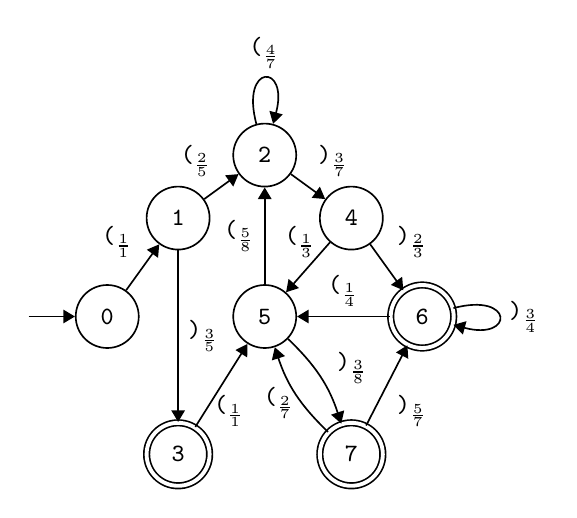
\begin{tikzpicture}[
  >=Triangle,
  font=\ttfamily\small,
  state/.style={
    circle,
    draw,
    minimum size=8mm,
    inner sep=0pt,
    semithick
  },
  final/.style={
    state,
    double,
    double distance=1.4pt
  },
  edge/.style={
    ->,
    semithick
  },
  every loop/.style={
    looseness=8,
    min distance=8mm
  }
]

% Manual, roughly square layout:
% left/right symmetry is used, but q5 is placed inside the shape
% so the automaton is not just a simple circular perimeter.
\node[state] (q0) at (-2.00,  0.00) {\statelabel{0}};
\node[state] (q1) at (-1.10,  1.25) {\statelabel{1}};
\node[state] (q2) at ( 0.00,  2.05) {\statelabel{2}};
\node[final] (q3) at (-1.10, -1.75) {\statelabel{3}};
\node[state] (q4) at ( 1.10,  1.25) {\statelabel{4}};
\node[state] (q5) at ( 0.00,  0.00) {\statelabel{5}};
\node[final] (q6) at ( 2.00,  0.00) {\statelabel{6}};
\node[final] (q7) at ( 1.10, -1.75) {\statelabel{7}};

% Invisible start point
\coordinate (start) at (-3, 0.00);

\path[edge]
  (start) edge (q0)

  (q0) edge node[above left]  {\(\mbox{(}_{\frac{1}{1}}\)} (q1)

  (q1) edge node[above left]   {\(\mbox{(}_{\frac{2}{5}}\)} (q2)
       edge node[right]        {\(\mbox{)}_{\frac{3}{5}}\)} (q3)

  (q2) edge[loop above] node  {\(\mbox{(}_{\frac{4}{7}}\)} (q2)
       edge node[above right] {\(\mbox{)}_{\frac{3}{7}}\)} (q4)

  (q3) edge node[below] {\hspace{0.2cm}\(\mbox{(}_{\frac{1}{1}}\)} (q5)

  (q4) edge node[above]  {\hspace{-0.2cm}\(\mbox{(}_{\frac{1}{3}}\)} (q5)
       edge node[above right] {\(\mbox{)}_{\frac{2}{3}}\)} (q6)

  (q5) edge node[left]        {\(\mbox{(}_{\frac{5}{8}}\)} (q2)
       edge[bend left=14] node[below left] {\hspace{-1cm}\(\mbox{(}_{\frac{2}{7}}\)} (q7)

  (q6) edge node[above]       {\(\mbox{(}_{\frac{1}{4}}\)} (q5)
       edge[loop right] node  {\(\mbox{)}_{\frac{3}{4}}\)} (q6)

  (q7) edge[bend left=14] node[above right] {\hspace{0.4cm}\(\mbox{)}_{\frac{3}{8}}\)}  (q5)
       edge node[below right] {\(\mbox{)}_{\frac{5}{7}}\)} (q6)
  ;

\end{tikzpicture}

\end{document}